\documentclass[conference,letterpaper,onecolumn]{IEEEtran}
%\usepackage[latin1]{inputenc}
%\usepackage[ansinew]{inputenc}
\usepackage[utf8]{inputenc}

\usepackage{graphicx}
\usepackage{psfrag}
\usepackage{stfloats}
%\usepackage[spanish]{babel}
\usepackage{epsfig}
\usepackage{pifont}
\usepackage{amssymb}
\usepackage{fixltx2e}
\usepackage{amsmath}
\usepackage{rotate}
\usepackage{anysize}
%\usepackage{rotating}
%\usepackage{fancybox}
\usepackage{float}
\usepackage{fancybox}
\usepackage{subfig}

\newcommand{\pig}[1]{\mbox{\boldmath ${#1}$}	}

\newtheorem{Theod}{{\bf Definici\'on}}

\setlength{\oddsidemargin}{5mm}
\setlength{\evensidemargin}{5mm}
\setlength{\topmargin}{4mm}
\setlength{\textwidth}{15cm}
\setlength{\columnsep}{5mm}
\setlength{\textheight}{24cm}





\begin{document}

\title{Double bounded bi-parameter homotopy applied to bipolar circuit simulation}

\author{\authorblockN{H\'ector V\'azquez-Leal}
\authorblockA{Universidad Veracruzana\\
Facultad de Instrumentaci\'on Electr\'onica\\
Xalapa, Veracruz, M\'exico\\
Email: hvazquez@uv.mx}
\and
\authorblockN{Arturo Sarmiento-Reyes}
\authorblockA{INAOE\\
Departamento de Electr\'onica\\
Email: jarocho@inaoep.mx}
\and
\authorblockN{Luis Hern\'andez-Mart\'{\i}nez}
\authorblockA{INAOE\\
Departamento de Electr\'onica\\
Email: luish@inaope.mx}
\and
\authorblockN{Roberto Casta\~neda Sheissa}
\authorblockA{Universidad Veracruzana\\
Facultad de Instrumentaci\'on Electr\'onica\\
Xalapa, Veracruz, M\'exico\\
Email: rocastaneda@uv.mx}
}

\maketitle

\begin{abstract}

En este trabajo se presenta una homotopia biparam\'etrica con criterio de paro automatizado.
La principal característica de esta homotopia biparam\'etrica es la de tener eje de simetría, doble l{\'i}nea
solución acotante, puntos de inicio y fin arbitrarios y un método para establecer la función biparam\'etrica.  Finalmente,
se ejemplificar su uso con un circuito no lineal (de benchmark) con múltiples puntos de operación.

\end{abstract}
 

\section{Introduction}

La solución de sistemas de ecuaciones no lineales es una necesidad imperante en diversas áreas de la física, en particular 
en el área de la electrónica la solución de sistemas de ecuaciones no lineales permite averiguar el
comportamiento aproximado de los circuitos integrados aun antes de ser fabricados, permitiendo así que los diseñadores
iteren y mejoren sus diseños a un bajo costo. El método mas utilizado es el método de Newton-Raphson (NR), el cual
es de convergencia cuadrática \cite{homo_ogrodzki,cont_quasi}. Sin embargo, debido a que el método es de convergencia local \cite{cont_quasi,Schwa_book}, no se puede garantizar que
el NR convergerá satisfactoriamente a alguna solución.  Por lo tanto, se crearon los métodos de homotopía, los cuales
tienen mejor convergencia que el método de NR.


\section{Homotopy}

Los m\'etodos de homotop\'{\i}a (tambien llamados m\'etodos de deformaci\'on continua)
no s\'olo son \'utiles en el \'area de an\'alisis en CD, si no que tambi\'en encuentran
aplicaci\'on en el \'area de an\'alisis de transiente \cite{homo_ArtificialP}, 
ingener\'{\i}a qu\'{\i}mica, psicolog\'{\i}a estad\'{\i}stica, econom\'{\i}a, f\'{\i}sica, etc.




Los m\'etodos de homotop\'{\i}a se fundamentan en el hecho de
que las so\-lu\-cio\-nes se encuentran conectadas por una curva, denominada
\emph{curva de so\-lu\-cio\-nes}. 
Para la obtenci\'on de esta curva se agrega
un par\'ametro adicional al sistema de ecuaciones original, lo cual
permite obtener la siguiente ecuaci\'on aumentada:

\begin{equation}
\pig{H}(\pig{f}(\pig{x}),\lambda )=\pig{0}
\label{homotopia}
\end{equation}
donde $\pig{H}$ representa la funci\'on de homotop\'{\i}a,
$\lambda$ el par\'ametro de continuaci\'on y
$\pig{f}(\pig{x})$ la ecuaci\'on original a resolver,
convirtiendo el problema original en un problema de integraci\'on
num\'erica \cite{homo_richter} en el que la variable de integraci\'on es el par\'ametro de
continuaci\'on $\lambda$.




Un esquema  de homotop\'{\i}a est\'a dado por:
\begin{equation}
\pig{H}(\pig{f}(\pig{x}),\lambda ) =
\pig{f}(\pig{x})-(1-\lambda )\pig{f}(\pig{x}_{0}) = 0
\label{hexampl}
\end{equation}
Cuando $\lambda =0$, se tiene una soluci\'on conocida {\em a priori}\,
en $\pig{x}_{0}$, usualmente una soluci\'on trivial.
Variando $\lambda$ desde 0 hasta 1, la soluci\'on
de esta ecuaci\'on se mueve desde $\pig{x}_{0}$ hasta la soluci\'on
de la ecuaci\'on $\pig{f}(\pig{x})=0$. 

Los m\'etodos de homotop\'{\i}a transforman el problema original
est\'atico en un problema din\'amico o transitorio \cite{homo_ogrodzki}.
Adem\'as, el problema din\'amico contiene todas las soluciones del
problema est\'atico original y te\'oricamente
permite encontrar todas las soluciones, lo cual no sucede en el problema
est\'atico \cite{homo_ogrodzki}.
Los m\'etodos de homotop\'{\i}a presentan problemas
debido a discontinuidades en la trayectoria homot\'opica o a puntos
de bi\-fur\-ca\-ci\'on \cite{homo_ogrodzki,homo_DWolfMulti}.
Sin embargo, existen nuevas propuestas de esquemas de
homotop\'{\i}a que pueden evitar estos problemas
\cite{homo_DWolfMulti}, como son las homotop\'{\i}as multiparam\'etricas.


\section{Multiparameter Homotopies}


La caracter\'{\i}stica b\'asica de una homotop\'{\i}a multiparam\'etrica
es la de agregar m\'as de un par\'ametro homot\'opico al sistema de NAEs \cite{homo_DWolfMulti}.
La homotop\'{\i}a multiparam\'etrica ($\pig{H}(\pig{x},\pig{\lambda}$)),
tiene una soluci\'on trivial cuando los par\'ametros de
homotop\'{\i}a tienen un valor de cero. Asimismo, cuando 
los par\'ametros de homotop\'{\i}a
tienen valor de uno, la funci\'on de homotop\'{\i}a se 
transforma a s\'{\i} misma en el sistema original de NAEs
($\pig{f}(\pig{x})$). La funci\'on de homotop\'{\i}a
multiparam\'etrica es:

\begin{equation}
\pig{H}(\pig{f}(\pig{x}),\lambda_1,\lambda_2,...,\lambda_n)=0, \qquad
\lambda_1,\lambda_2,...\lambda_n\quad \in[0,1]
\end{equation}
donde $n$ es el n\'umero de par\'ametros de homotop\'{\i}a 
y  $\pig{x}$ es el vector de inc\'ognitas.


Estos m\'etodos se han estudiado con la finalidad
de saber en qu\'e pueden ayudar para evitar bifurcaciones \cite{homo_DWolfMulti},
pliegues agudos, soluciones infinitas,
caminos abreviados (abbreviated paths), curvas
de soluci\'on cercanamente espaciadas y ramas
desconectadas en la curva de soluci\'on \cite{homo_DWolfMulti}.

La homotop\'{\i}a multiparam\'etrica aplicada a circuitos se puede visualizar como la
deformaci\'on del circuito a un circuito reducido, de tal forma que al barrer
los par\'a\-me\-tros homot\'opicos se van obteniendo circuitos cada vez m\'as similares
al original. Por lo tanto, este tipo de procedimiento garantiza una suave convergencia
a la soluci\'on final pues empieza por resolver un circuito reducido y cada vez m\'as aumentado cada vez m\'as cercano al circuito original. Por lo tanto, esta es la raz\'on de mejor convergencia
de la homotop\'{\i}a con respecto a m\'etodos como el de Newton-Raphson.

Supongase que se cuenta con un circuito de 3 componentes conectados en serie: una fuente de voltaje $V_1$,
un resistencia $R_1$ y un resistor no lineal $K_1$ cuya relacion  de rama es:

\begin{displaymath}
i=u^2
\end{displaymath}


A este circuito no lineal se le aplica una homotop\'{\i}a
multiparam\'etrica de tal forma que la expresi\'on para $K1$
se transforma como sigue:

\begin{displaymath}
i=\lambda_2 u^{2\lambda_1}
\end{displaymath}

La homotop\'{\i}a usa dos par\'ametros  $\lambda_1$ y $\lambda_2$,
los cuales son barridos en el rango de  [0,1]. El barrido
de cada par\'ametro puede ser representado por circuitos 
equivalentes como se observa en la figura \ref{homos}. El total de
circuitos intermedios es de nueve, usando s\'olo tres 
pasos
por cada par\'ametro.
Debido a que el efecto de los par\'ametros homot\'opicos
se concentra en el resistor no lineal del circuito $K1$, cada
circuito equi\-va\-lente s\'olo se ve modificado en dicho componente.
A continuaci\'on se presenta una breve explicaci\'on
de cada circuito equivalente:

\begin{itemize}
\item Caso \ding{172} donde $[\lambda_1, \lambda_2]=[0,0]$.

El circuito equivalente es un circuito abierto.
\item Caso \ding{173} donde $[\lambda_1, \lambda_2]=[0,0.5]$.

El resistor no lineal se comporta como una fuente de corriente constante.
\item Caso  \ding{174} donde $[\lambda_1, \lambda_2]=[0,1]$

El resistor no lineal se comporta como una fuente de corriente constante, pero
de mayor valor que en el paso \ding{173}.
\item Caso  \ding{175} donde $[\lambda_1, \lambda_2]=[0.5,0]$ 

El circuito equivalente es un circuito abierto.
\item Caso  \ding{176} donde $[\lambda_1, \lambda_2]=[0.5,0.5]$

 El resistor no lineal se comporta como una resistencia lineal positiva, por lo que
el circuito equivalente es una fuente en serie con 2 resistencias lineales.
\item Caso  \ding{177} donde $[\lambda_1, \lambda_2]=[0.5,1]$ 

Sucede lo mismo que en el paso \ding{176}, pero la resistencia tiene mayor valor.
\item Caso  \ding{178} donde $[\lambda_1, \lambda_2]=[1,0]$ 

El circuito equivalente es un circuito abierto.
\item Caso  \ding{179} donde $[\lambda_1, \lambda_2]=[1,0.5]$ 

En este paso el circuito es ya bastante similar al circuito original. El resistor
no lineal es un polinomio.
\item Caso  \ding{180} donde $[\lambda_1, \lambda_2]=[1,0.5]$ 

En este paso el circuito es id\'entico al circuito original.
\end{itemize}


La homotop\'{\i}a sigue los pasos \ding{172},\ding{173}, \ding{176}, \ding{177} y  \ding{180} para completar la trayectoria a la primera soluci\'on.

Este ejemplo muestra como la homotop\'{\i}a multiparam\'etrica puede ser interpretada
como una deformaci\'on circuital. Este aspecto es de mucho inter\'es pues es posible
crear homotop\'{\i}as {\it ad hoc} para la soluci\'on de cirtuitos caracterizados
por no linealidades muy espec\'{\i}ficas, como circuitos compuestos por transistores MOS o Bipolares.
En estos casos es posible aplicar homotop\'{\i}as multiparam\'etricas a los modelos
de los transistores en forma an\'aloga al ejemplo anterior con la finalidad
de obtener trayectorias homot\'opicas m\'as suaves y por lo tanto mejorar la convergencia.


\begin{figure}[hbtp]
\centerline{
\epsfxsize=11cm
\epsffile{fig/circus1.eps}}
\caption{Interpretaci\'on circuital de la homotop\'{\i}a multip\'arametrica }
\label{homos}
\end{figure}

\section{homotopia biparametrica doblemente acotada}

Es posible formular una homotopia multiparametrica con criterio de paro, utilizando
la homotopia polinomial doblemente acotada cuya formulación es:

\begin{equation}
{\small
\begin{array}{l}
\pig{H}(\pig{f}(\pig{x}),\lambda_1 )=\lambda_1(\lambda_1-a)(x-x_i)(x-x_f) -C(\lambda_1-a/2)^2 \pig{f}(\pig{x})^2
\end{array}}
\label{homotopiaP}
\end{equation}

where $\lambda_1$ is the homotopy parameter, $a$ is a constant that represents the separation between solution lines, $x_i$ is the initial point, $x_f$ the final point, and $C$ an arbitrary constant.


Ahora se introduce un segundo parametro homotopico de tal modo que la homotopia se reformula como:

\begin{equation}
{\small
\begin{array}{l}
\pig{H}(\pig{f}(\pig{x}),\lambda_1 )=\lambda_1(\lambda_1-a)(x-x_i)(x-x_f) -C(\lambda_1-a/2)^2 \pig{f}(\pig{x},\lambda_2)^2
\end{array}}
\label{homotopiaPx1}
\end{equation}

donde $\pig{f}(\pig{x},\lambda_2)$ representa la introducción del segundo parámetro homotopico ($\lambda_2$) dentro de la ecuación de
equilibrio $f(x)$.

En este trabajo se considera que la ecuación de equilibrio esta formulada mediante el método del análisis nodal modificado (MNA),
el cual establece que existe un vector estimulo, el cual contiene la contribución de  las fuentes de corriente independientes
y las fuentes de corriente no lineales. En circuitos con transistores bipolares el modelo de Ebbers-Mol se basa en la interconexi\'on de de fuentes controladas y de diodos cuya relación de rama es una función exponencial.

Actualmente, el MNA y sus variantes son los métodos m\'as usados dentro de programa de simulación
de circuitos.
La idea del método MNA es considerar las corrientes de ramas de los
elementos no NA-compatibles como variables adicionales y sus correspondientes
relaciones de rama como ecuaciones adicionales. La nuevas
variables están disponibles como incógnitas adicionales.

\begin{equation}
\left[ \begin{array}{c}
MNA
\end{array} \right]
\left[ \begin{array}{c}
\pig{v} \\
\pig{i} \\
\end{array} \right]
=
\left[ \begin{array}{c}
\pig{i_{cts}}
\end{array} \right]
+
\left[ \begin{array}{c}
\pig{i_{nlin}}
\end{array} \right]
\end{equation}
donde $MNA$ representa la contribuciones de las conductancias y relaciones de rama de los elementos no-NA compatibles,
$\pig{v}$  es vector de incógnitas el cual representa los voltajes de todos los nodos del circuito, $\pig{i}$ es otro vector de incógnitas el cual representa las corrientes de los elementos no-NA compatibles, $\pig{i_{cts}}$ representa las contribuciones
al vector estimulo de todas las fuentes de corriente constantes, y de las caídas de potencial en los elementos no-NA compatibles (fuentes de voltaje constantes o fuentes de voltaje controladas), y finalmente $\pig{i_{nlin}}$ representa todas las contribuciones de las fuentes de voltaje y de corrientes no lineales.

Resulta interesante observar que el vector $\pig{i_{nlin}}$ contiene la suma total de las contribuciones no lineales
de los elementos de un circuito. En un circuito con transistores bipolares el modelo de Ebers-Mol contiene
diodos cuyo modelo m\'as simple es una fuente de corriente no lineal la cual depende exponencialmente de la caida de potencial del diodo. Por lo tanto, la relación de rama de los diodos del modelo Ebers-Mol terminaran en el vector estimulo $\pig{i_{nlin}}$.

Cuando se realiza la deformación del parámetro homot\'opico desde cero hasta uno, lo que se esta haciendo es resolver
inicialmente un problema de solución trivial, continuando con una deformación continua que gradualmente
aumenta la no linealidad de la función homot\'opica $H(f(x),\lambda)$ hasta que en $\lambda=1$, $H(f(x),\lambda)$ es igual a $f(x)=0$.
Asimismo, al agregar el par\'ametro homot\'opico  a la ecuación de equilibrio se debe buscar que la trayectoria homot\'opica sigua un camino lo m\'as suavizado posible para no tener problemas como sharp folds; esto se puede lograr multiplicando $\lambda$ por cada termino no lineal como funciones exponenciales, logaritmos naturales, funciones cuadráticas, etc.
Por lo tanto, en este trabajo se plantea multiplicar $\lambda_2$ por el vector estimulo $\pig{i_{nlin}}$, con la finalidad
de eliminar las no linealidades de la ecuacion de equilibrio en $\lambda_2=0$. La funcion homotopica \ref{homotopiaPx1} se reescribe como:

\begin{equation}
{\small
\begin{array}{l}
\pig{H}(\pig{f}(\pig{x}),\lambda_1 )=\lambda_1(\lambda_1-a)(x-x_i)(x-x_f) -C(\lambda_1-a/2)^2 \pig{f}(\pig{x},\lambda_2\pig{i_{nlin}})^2
\end{array}}
\label{homotopiaPx3}
\end{equation}

La función homot\'opica $H$ es una función de $n+2$ variables con $n$ ecuaciones, donde $n$ es igual al n\'umero total de nodos
mas el n\'umero de elementos no-NA compatibles. Por lo tanto es necesario agregar una ecuación extra con la finalidad
de poder utilizar las técnicas convencionales de trazado de trayectorias homot\'opicas. 
La ecuacion es una relacion de $\lambda_1$ y $\lambda_2$ la cual denominaremos $G(\lambda_1,\lambda_2)=0$.
Dicha ecuacion debe tener dos puntos obligados de cruce $\lambda_i=[\lambda_1,\lambda_2]=[0.5,0]$ y $\lambda_s=[\lambda_1,\lambda_2]=[1,1]$. De tal modo que $\lambda_i$ es el punto donde la solución del circuito es trivial ($x_i$) y  $\lambda_s$
es el punto donde la solución de $H$ es exactamente la solución buscada de la ecuación de equilibrio $f(x_s)=0$.
Se debe notar que la excursión de $\lambda_1$ inicia normalmente en 0.5 ya que por normalizaci\'on el eje de simetría
se establece con $a=1$. Sin embargo, los puntos intermedios de la trayectoria homotopica $\lambda_1-\lambda_2$ no estan definidos y juegan un papel
importante en la suavidad de la trayectoria homotopica completa. En este trabajo se propone la siguiente ecuacion como la ecuacion de la trayectoria homotopica
en $\lambda_1-\lambda_2$:


\begin{equation}
\begin{array}{l}
\lambda_{{1}}={ \left( \lambda_{{2}}+{\frac {B \left( - 1+A \right) }
{AB+ 1- 2A}} \right) \over  \left( -{\frac { \left( - 1+ 2\,
A- B \right) \lambda_{{2}}}{AB+ 1- 2A}}+ 2\,{\frac {B
 \left( - 1+A \right) }{AB+ 1- 2A}} \right) }
\end{array}
\label{homotopiaPx4}
\end{equation}

donde $[\lambda_1,\lambda_2]=[A,B]$ es el punto donde cruza la curva de la funci\'on de $\lambda_1-\lambda_2$

\begin{figure}[hbtp]
\psfrag{o}{$\lambda$}
\centering
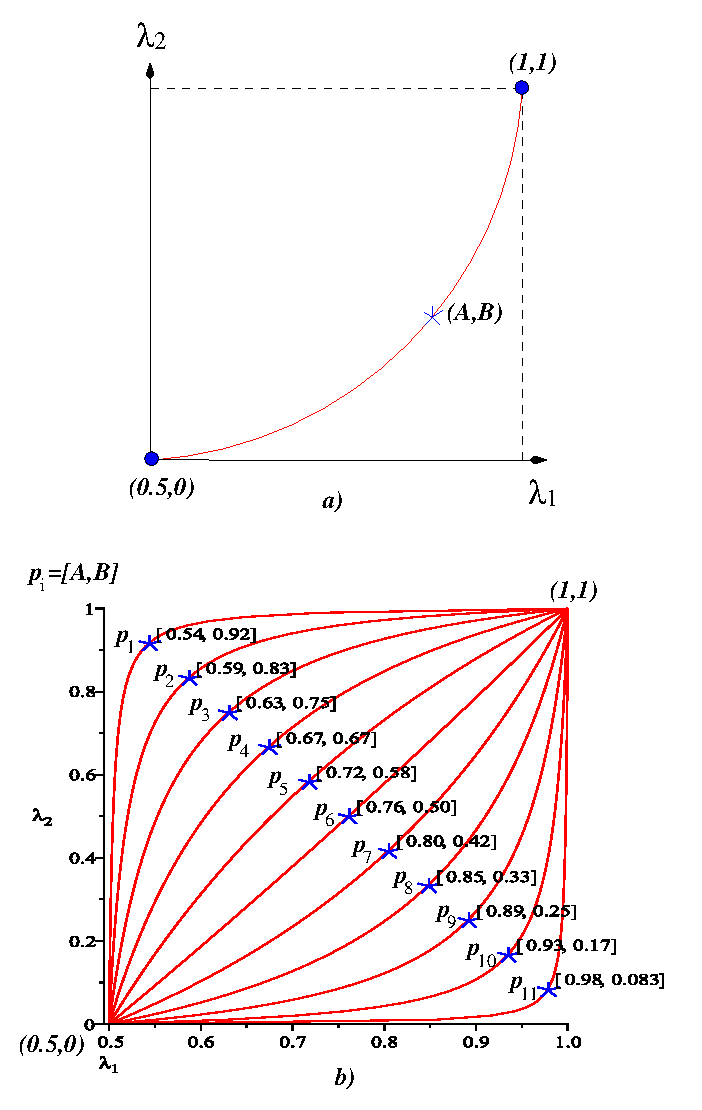
\includegraphics[scale=0.55]{fig/curvasl.eps}
\caption{Trayectoria  de $\lambda_1-\lambda_2$}
\label{curvasl}
\end{figure}



Homotopy can be expressed in general way as (using $a=1$):

\begin{displaymath}
\pig{H}(\pig{f}(\pig{x}),\lambda_1,\lambda_2\pig{i_{nlin}} ) = \left\{\begin{array}{rl}
f(x^*)=0 & \textrm{for  $\lambda_1=1, \lambda_2=1$ and $x=x^*$}\\
(x-x_i)(x-x_f)=0 & \textrm{for $\lambda_1=0.5$ and $\lambda_2=0$}\\
f(x^*)=0 & \textrm{for $\lambda_1=1, \lambda_2=1$ and $x=x^*$}
\end{array}\right.
\end{displaymath}


En otras palabras, se puede decir que:
\begin{itemize}
\item For $\lambda_1=0.5(a+b)$ and $\lambda_2=0$ the solution of $H^{-1}(0)$ is known or easy to obtain using computers. This point is known as Homotopy's initial point ($\lambda_i$).
\item For $\lambda_1=a$ and $\lambda_2=1$, $\pig{H}(\pig{f}(\pig{x}),\pig{a} )=\pig{f}(\pig{x})$. Means that at $\lambda_1=a$ and $\lambda_2=1$ all the solutions for $\pig{f}(\pig{x})$ are located.
\item For $\lambda_1=b$ and $\lambda_2=1$, $\pig{H}(\pig{f}(\pig{x}),\pig{b} )=\pig{f}(\pig{x})$. This means that at $\lambda_1=b$ and $\lambda_2=1$ all the solutions for $\pig{f}(\pig{x})$ are located.
\item The path for $\pig{H}^{-1}(\pig{0})$ is a continuous function of $\lambda$ within the range of $a \leq \lambda_1 \leq b $ and $0 \leq \lambda_2 \leq 1 $. 
\end{itemize}


Ya que $\lambda_2$ no interfiere directamente con la formulacion homotopica, solo afectando la ecuacion de equilibrio $f(x)$ y agregando una ecuacion extra al sistema, por lo tanto,
el resto de las propiedrades de esta homotopia multiparametrica concide con la homotopia reportada en [], como lo es: ramas simetricas, eje de simetria, punto de inicio
y punto final de la trayectoria homotopica y criterio de paro. Ahora se discutira una ejemplo de aplicacion de esta nueva homotopia.


\section{Study case: Circuit with bipolar transistors and a diode}


A circuit with bipolar transistors and a diode was reported in \cite{homo_tadeusiewicz} and  \cite{homo_yamamurawise}, it was solved using piecewise methods. Then, in \cite{homo_yamamura}, the circuit was resolved using modified fixed point Homotopy. This circuit has 3 operating points. The Ebers-Moll is used for all the transistors. The equation for the model is given as:

\begin{displaymath}
\left[ \begin{array}{c}
i_{D_E} \\
i_{D_C}
\end{array}\right] =
\left[ \begin{array}{cc} 1  & \alpha_R \\
\alpha_F & 1 \\
\end{array}\right] \left[ \begin{array}{c}
10^{-9}(e^{(40v_{be})} - 1) \\
10^{-9}(e^{(40v_{bc})} - 1)
\end{array}\right]
\end{displaymath}

As for the diode, the model is:

\begin{displaymath}
i_d=10^{-9}(e^{40u} - 1)
\end{displaymath}

\begin{figure}[hbtp]
\centerline{
\epsfxsize=95mm
\epsffile{yamamura/diotran.eps}
\hspace{3mm}
\epsfxsize=30mm
\epsffile{yamamura/y2.eps}
}
\caption{Circuit with bipolar transistors and a diode.}
\label{yamamuracircuito}
\end{figure}

First, the equilibrium equation is formulated using the modified nodal analysis with the result of a system having 14 equations and 14 variables. The circuit is shown in figure \ref{yamamuracircuito}.


Now, DBH is applied to solve the circuit; the Homotopy formulation is expressed as follows:

\begin{displaymath}
\begin{array}{c}
H_1(f_1,\lambda)=\lambda(\lambda+1)(\lambda-1)(\lambda-2)(v_1-13)(v_1+13)+C(\lambda-0.5)^2 f_1^2=0\\
H_2(f_2,\lambda)=\lambda(\lambda+1)(\lambda-1)(\lambda-2)(v_2-13)(v_2+13)+C(\lambda-0.5)^2 f_2^2=0\\
\vdots \\
H_{14}(f_{14},\lambda)=\lambda(\lambda+1)(\lambda-1)(\lambda-2)(I_E-13)(I_E+13)+C(\lambda-0.5)^2 f_{14}^2=0\\
\end{array}
\end{displaymath}

where the constant value $C=1$, the bounding lines are $a=0$ and $b=1$, and the initial point $x_i$ for the Homotopy path is selected as shown in figure \ref{yamaie}(c).

So, the next step is to solve the circuit using the double bounded Homotopy, resulting in the convergence to the three known solutions for the circuit (figure \ref{yamaie}(c)). The Homotopy path correspondent to the nodal voltage $v_2$ is displayed in figures \ref{yamaie}(a) and \ref{yamaie}(b). Finally, the final point $x_f$ for the Homotopy trace is exhibited in figure \ref{yamaie}(c).




\begin{figure}[hbtp]
\centerline{
\epsfxsize=105mm
\epsffile{fig/yamamu.eps}
}
\caption{Homotopy trajectory}
\label{yamaie}
\end{figure}


\begin{table}[hbtp]
{\small
\center{
\hspace{-4mm}
\begin{tabular}{||c|c|c|c|c|c|c|c|c|c|c|c|c|c|c||}
\hline\hline
Sol & $v_1$ & $v_2$ & $v_3$ & $v_4$ & $v_5$ & $v_6$ & $v_7$ & $v_8$ & $v_9$ & $v_{10}$& $v_{11}$ & $v_{12}$ & $v_{13}$ & $i_E$ \\ \hline
$S_1$ &  12 & 5.995 & 0.085 &0.368 &0.712 &0.436 &0.390 &0.699 &11.635 &0.4e-5 &0.039 &0.039 &0.321 &-0.0089 \\ \hline
$S_2$ & 12 & 0.883 & 0.278 &0.590 &0.631 &0.812 &0.315 &1.074 &11.647 &0.4e-5 &0.039 &0.039 &0.321 &-0.0100 \\ \hline
$S_3$ & 12 & 0.405 & 0.366 &0.685 &0.349 &6.796 &0.070 &7.038 &11.839 &0.4e-5 &0.039 &0.039 &0.321 &-0.0085 \\ \hline \hline
\end{tabular}
}
}
\caption{Operating points (solutions) for figure \ref{yamamuracircuito}. at $\lambda_1=1$ and $\lambda_2=1$}
\label{yamamuracircuitosoluc}
\end{table}

\begin{table}[hbtp]
{\tiny
\center{
\hspace{-4mm}
\begin{tabular}{||c|c|c|c|c|c|c|c|c|c|c|c|c|c|c|c|c||}
\hline\hline
Points & Iterations & Turning Points&$v_1$ & $v_2$ & $v_3$ & $v_4$ & $v_5$ & $v_6$ & $v_7$ & $v_8$ & $v_9$ & $v_{10}$& $v_{11}$ & $v_{12}$ & $v_{13}$ & $i_E$ \\ \hline
$x_i$ & - & - &+13 & +13& +13& -13& +13& +13& +13& +13& +13& +13& +13& +13& -13& -13  \\ \hline
$xf_{B_1}$ & 16669 & 11&+13& +13& +13& -13& +13& +13& +13& +13 & +13& +13&+13&+13&-13&+13   \\ \hline
$xf_{B_2}$ & 17063 &11 & +13 & -13 & +13 &-13& +13&  +13& +13& +13& +13& +13& +13& +13& -13& +13    \\ \hline
$xf_{B_3}$ & 16508 &11 &+13& +13 & +13& -13& +13& +13& +13&+13& +13& +13& +13& +13& -13 &+13  \\ \hline \hline
\end{tabular}
}
}
\caption{Punto de inicio  y final correspondiente a cada funcion multiparametrica ($B_1$, $B_2$ y $B_3$), considerando $\lambda_1=0.5$ and $\lambda_2=0$. }
\label{yamamuracircuitosoluc}
\end{table}





\section{Conclusions}

A new kind of Homotopy was presented, it is named double bounded algebraic Homotopy, which contains just 2 solution lines. It was demonstrated the symmetry of the Homotopy paths. 
Additionally, it was illustrated the use of Homotopy in a benchmark circuital case, showing its potential to be employed in analysis of non-linear circuits.

\bibliographystyle{amsplain}
\bibliography{carta}

\end{document}
